\section{Experiment Setup}

The BG-2 Pohl resonator consists of two main parts: a vibrometer and a control
box. The vibrometer is shown in Figure 2. A copper balance wheel is mounted on a
supporting frame, and the axis of the balance wheel is attached to the
supporting frame with a scroll spring. The spring provides an elastic restoring
torque to the wheel, which makes the balance wheel rotating about an equilibrium
position. 

\begin{figure}[H]
\centering
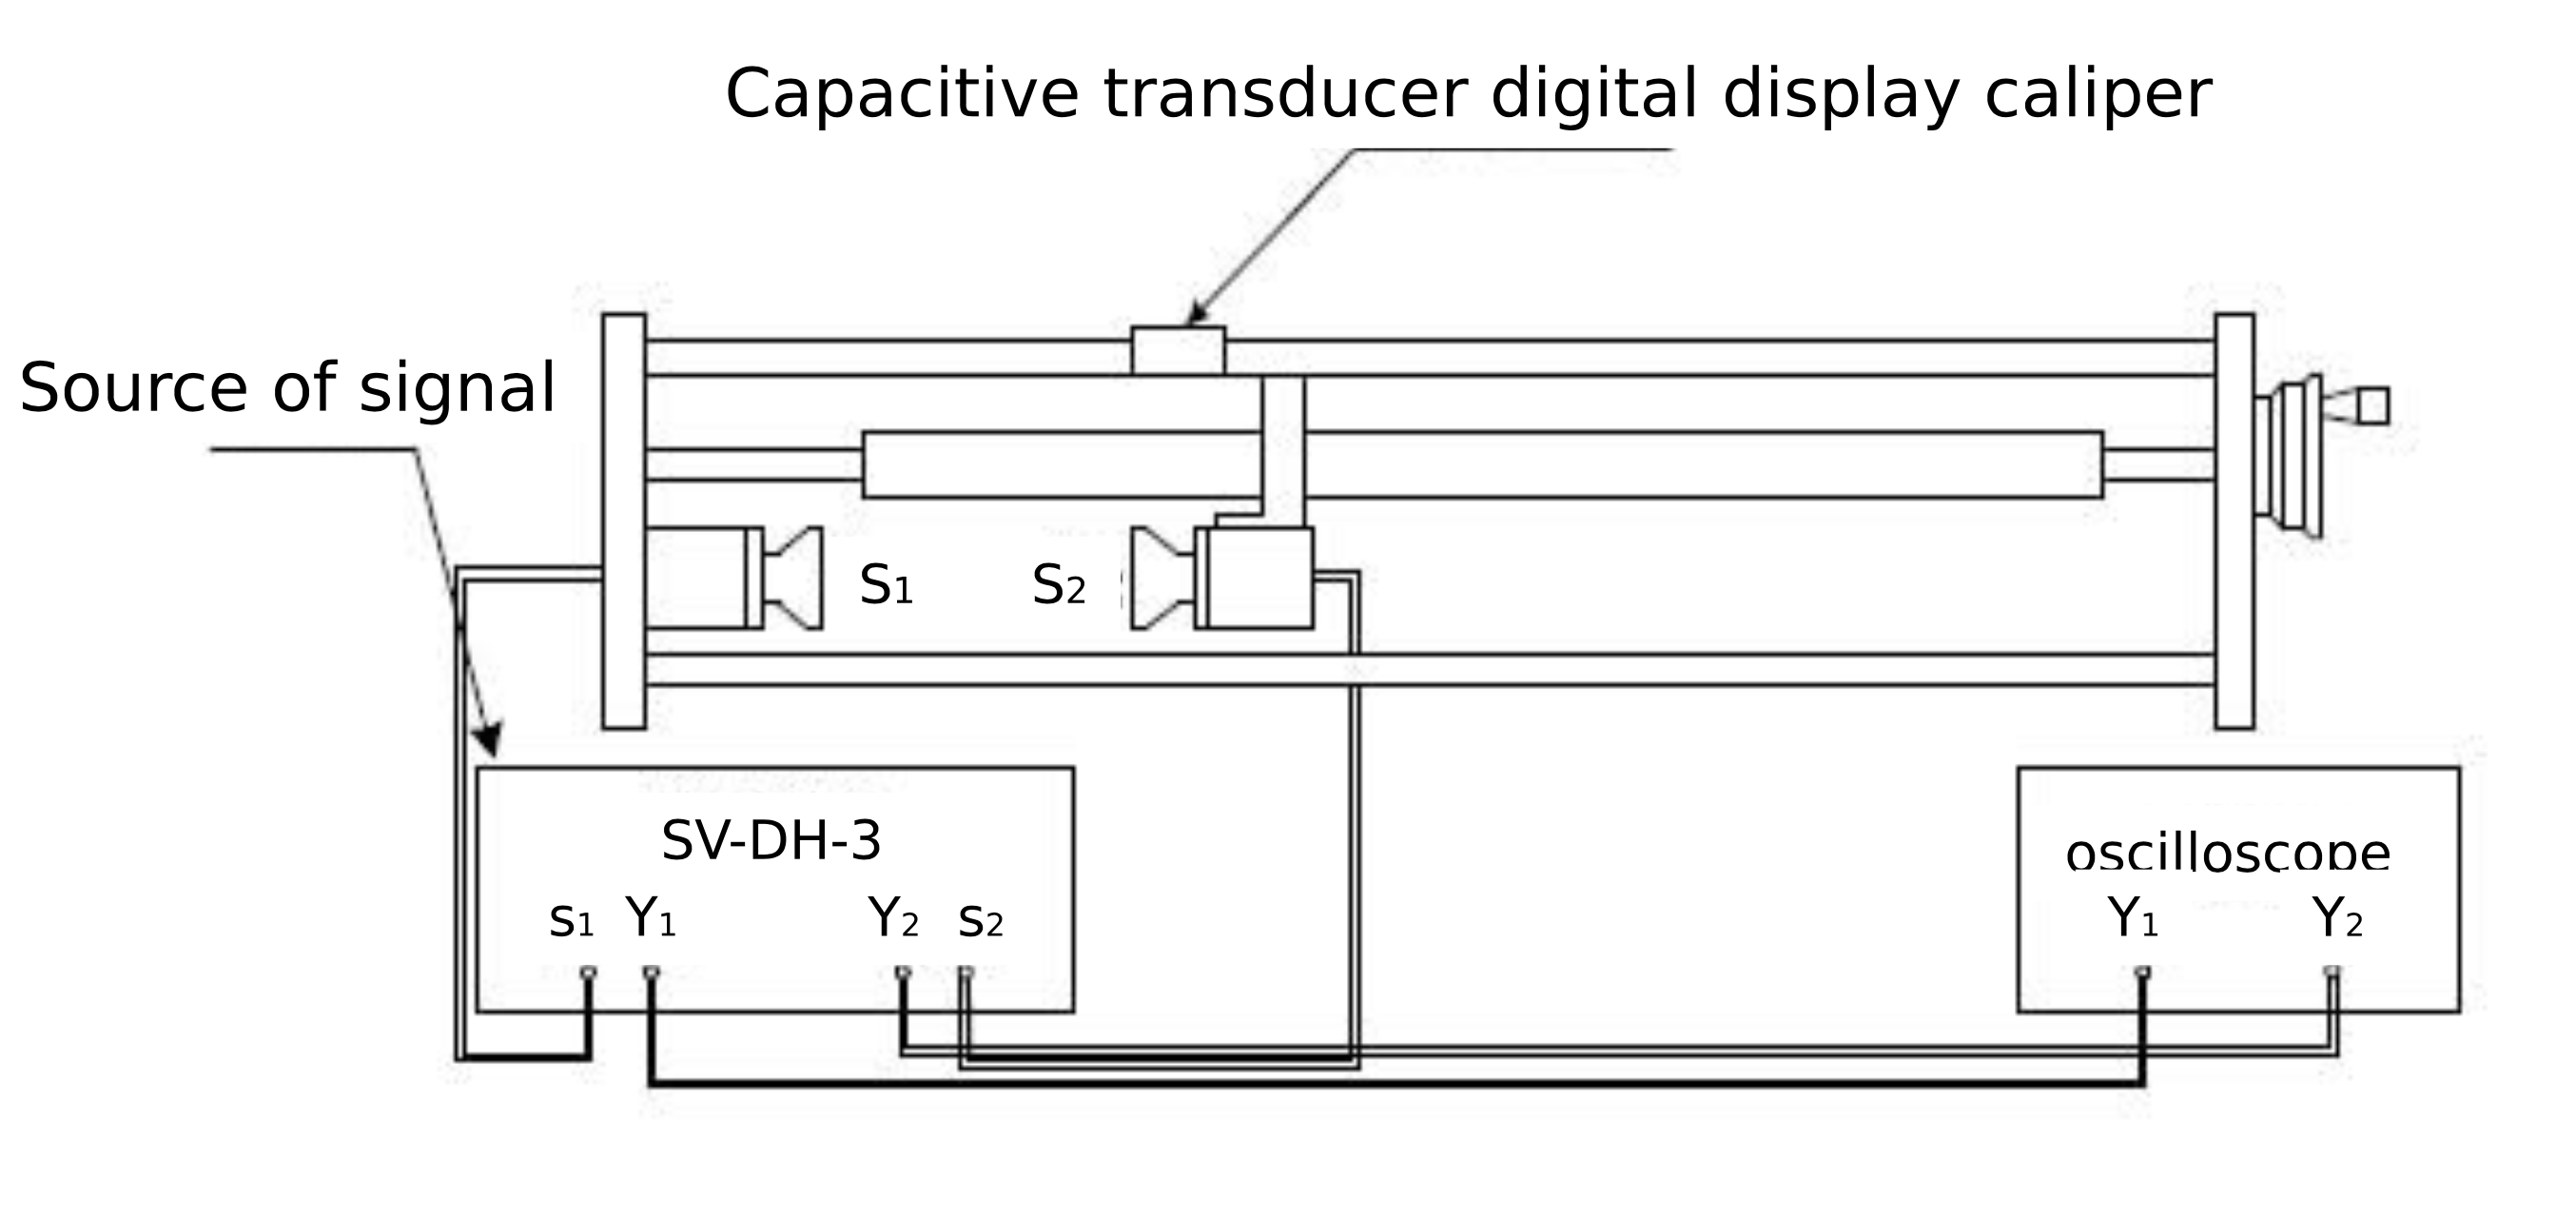
\includegraphics[width=0.9\textwidth]{fig/es1}
\caption{The dependence of the amplitude (left) and phase shift (right) of
  steady-state driven oscillations}
\label{aps} 
\end{figure}

There are many notches on the edge of the balance wheel with one notch being
much deeper than the others. A photoelectric detector is set above the deep
notch. The detector is used to measure the amplitude and the period of
oscillations, and it is connected to the electronic control box. 

A pair of coils is placed at the bottom of the supporting frame, with the
balance wheel fitting exactly into the gap between the two coils. Due to
electromagnetic induction, the wheel will be acted upon an electromagnetic
damping force when the coils are carrying current, and the magnitude of the
damping force can be controlled by changing the current. 

The device is equipped with a motor with an electric wheel and a rod used to
drive the wheel.
There is a Period Selection switch and a Period of Driving Force knob on the
electric control box, which allow to control the speed of the motor precisely. 
Another photoelectric detector is set above the turntable and connected to the
control box to measure the period of driving force. 

The phase shift can be measured using the glass turntable with an angle scale
and a strobe light.
The strobe is controlled by the photoelectric detector above the wheel. 
When the deep notch passes the equilibrium position, the detector
sends a signal and the strobe flashes.
In a steady state, a line on the angle scale will be highlighted by the flash of
the strobe and the phase difference can be read from the angle scale directly. 

The amplitude of oscillations is measured by counting the notches on the wheel,
and this measurement is performed by a photoelectric detector with the result
displayed on the electronic control box. 

\begin{figure}[H]
\centering
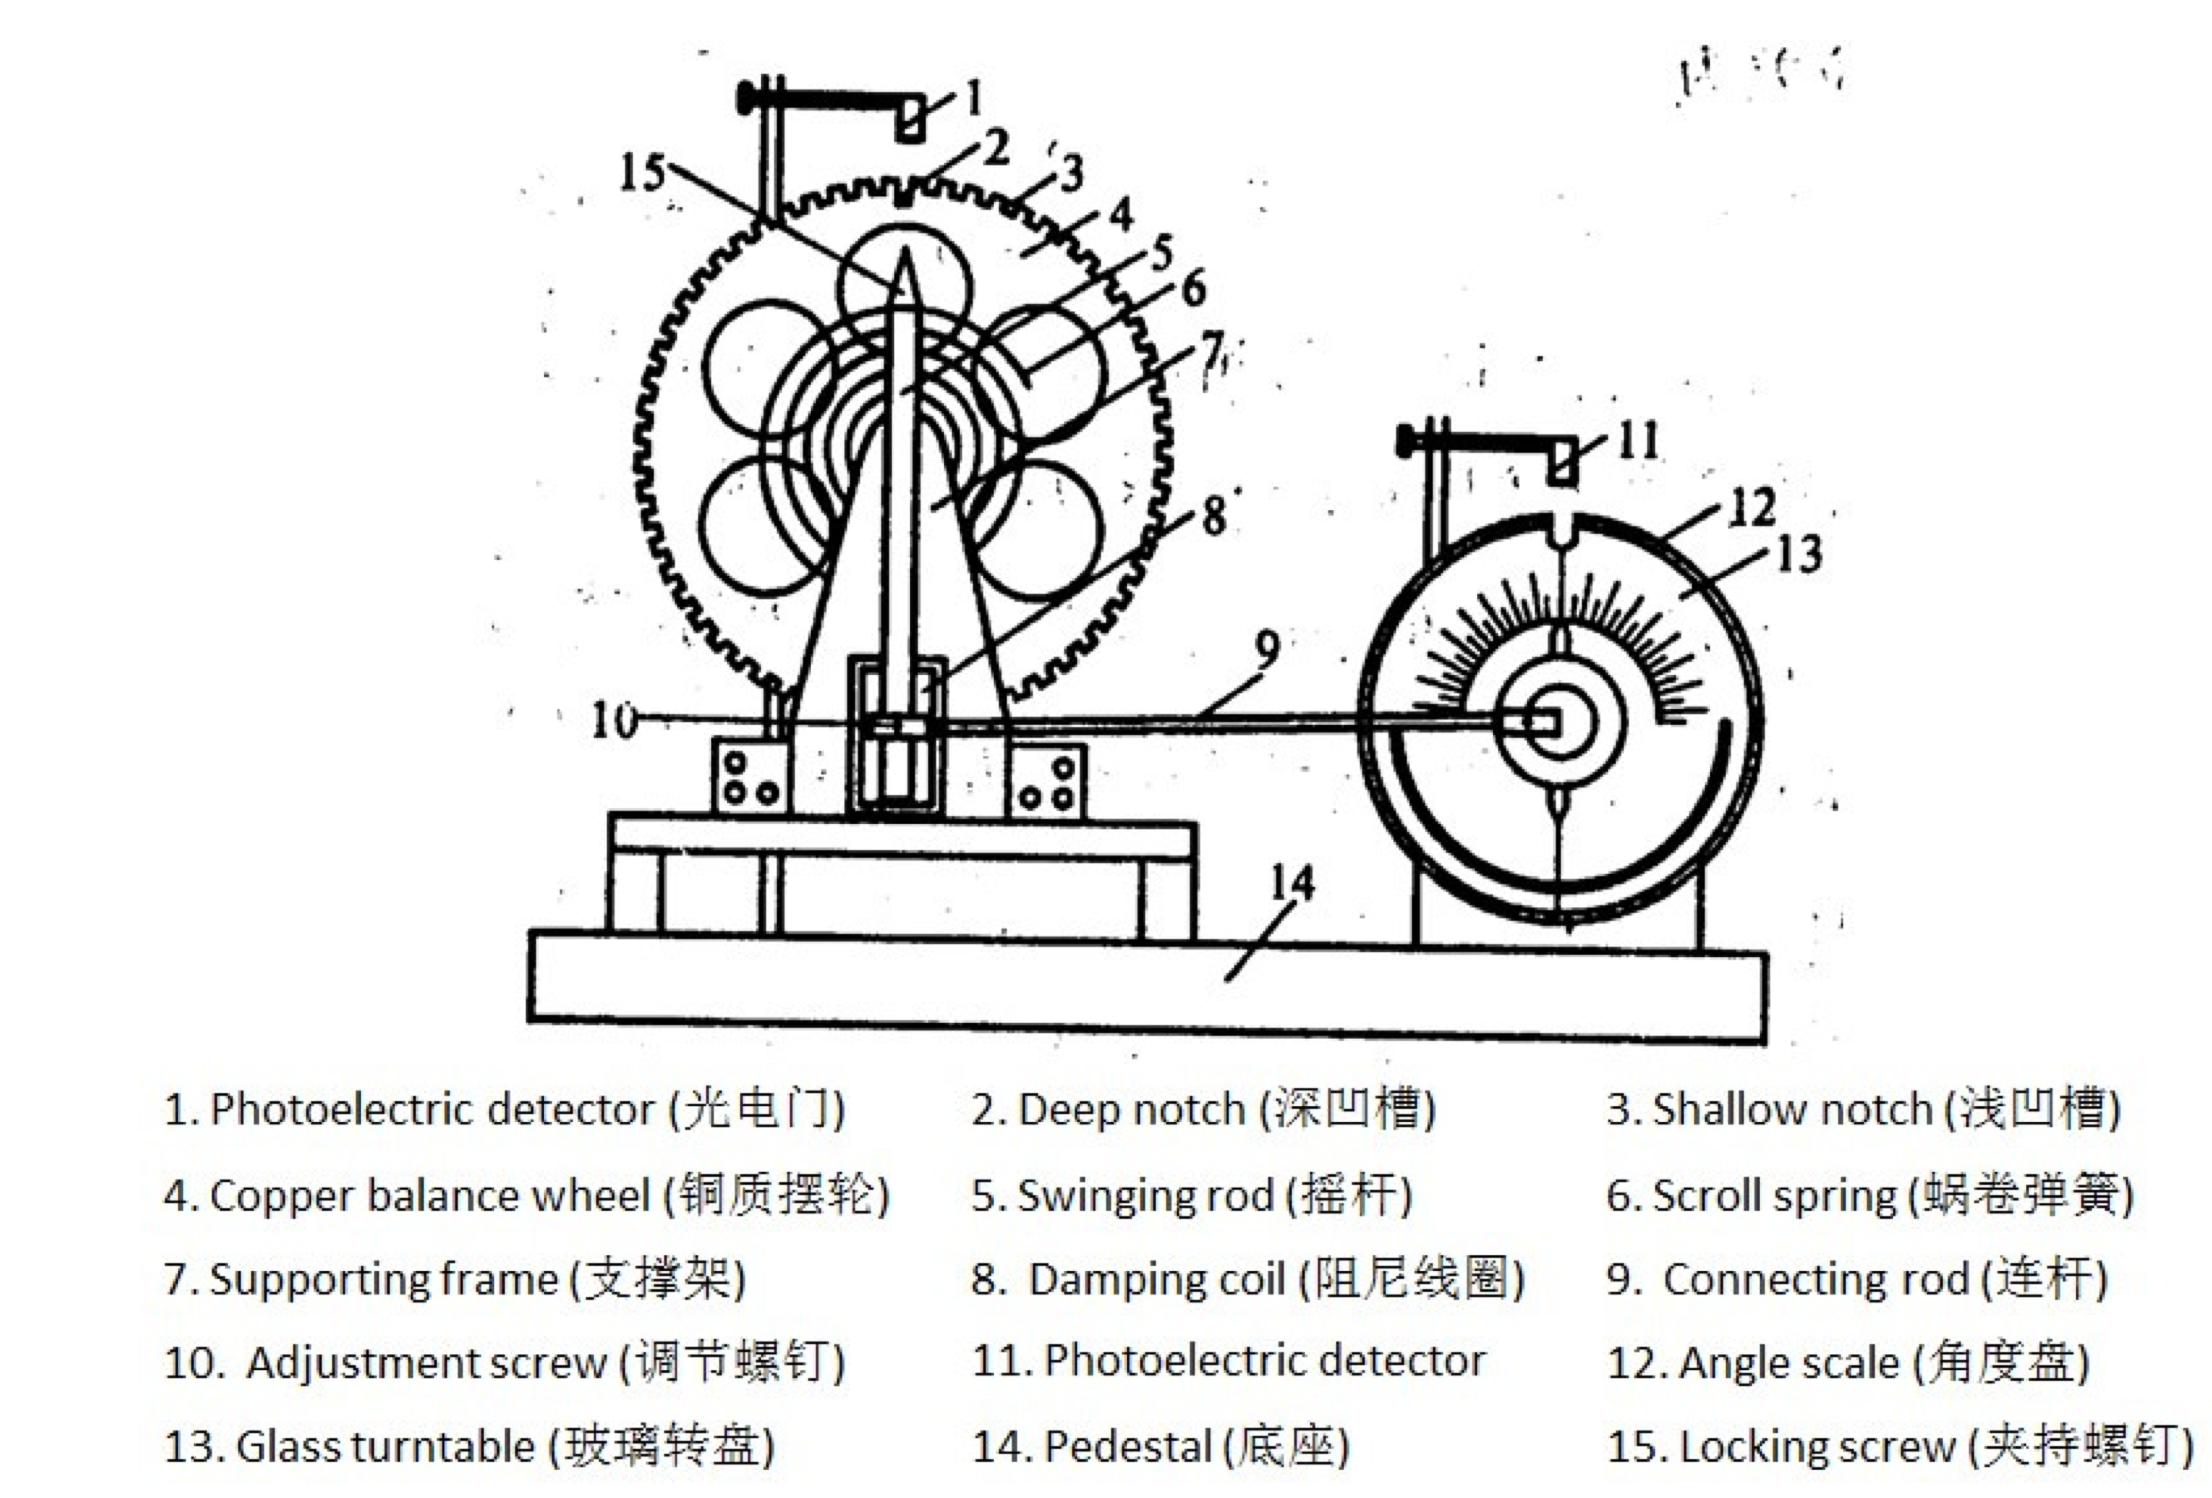
\includegraphics[width=0.9\textwidth]{fig/es2}
\caption{Vibrometer}\label{vib}
\end{figure}

The function Amplitude Display shows the oscillation amplitude of the balance
wheel and Period Display shows the oscillation period in two modes.
When the Period Selection switch is at position ``1'' , a single oscillation
period will be displayed; when the Period Selection switch is at ``10'', the
time of 10 oscillation periods will be displayed.
The reset button works only when the
Period Selection button is at ``10''. 
    
The period of the driving force can be changed precisely by using the Period of
the driving force knob, but please pay attention that the scale on the knob is
not very accurate. 

The Damping Selection knob changes the damping force by adjusting the electric
current through the coils at the bottom of the wheel.
There are six options, ranging from ``0'' (no current) to ``5'' (current of
about 0.6 A). Here we use ``2'', ``3'' or ``4''. 

The strobe generates a flash that allows you to read the phase difference from
the angle scale directly.
To protect the strobe, you should turn on the Strobe switch only when measuring
the phase difference.

The Motor Switch is used to control the motor.
You should turn the motor off when measuring the damping coefficient and the
natural angular frequency.

\begin{figure}[H]
\centering
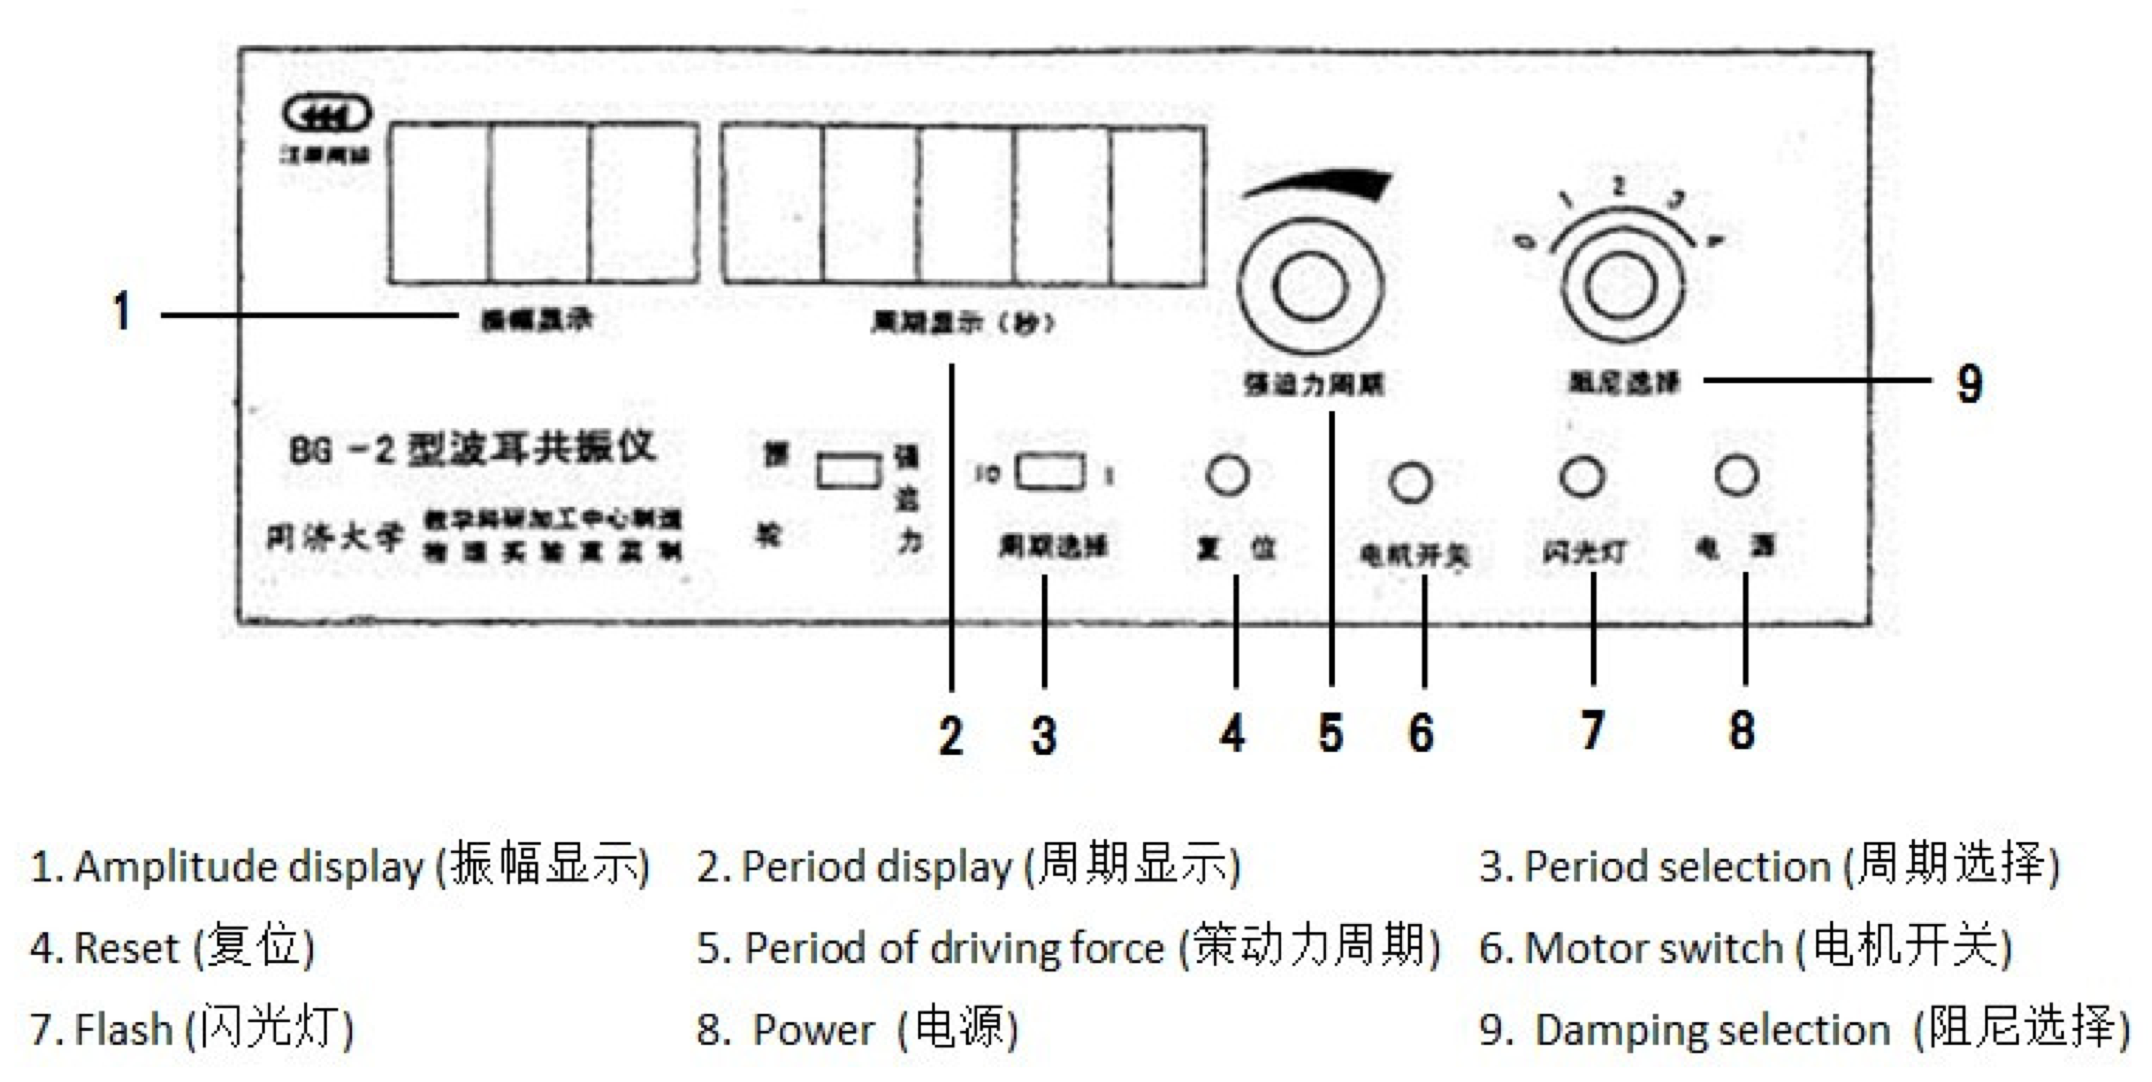
\includegraphics[width=0.8\textwidth]{fig/es3}
\caption{The front panel of the control box}
\label{panel}
\end{figure}

\subsection{Devices precision}
The precisions of the devices are shown in Table~\ref{precision}.

\begin{table}[H]
\centering
\begin{tabular}{|l|c|c|}
\hline
Devices & Precision & Unit\\ \hline
Timer on BG-2 Pohl resonator & 0.001 & [s]\\ \hline
Angle on BG-2 Pohl resonator & 1 & [$\degree$]\\ \hline
\end{tabular}
\caption{Devices precision}
\label{precision}
\end{table}